% Created by tikzDevice version 0.12 on 2019-04-30 14:04:59
% !TEX encoding = UTF-8 Unicode
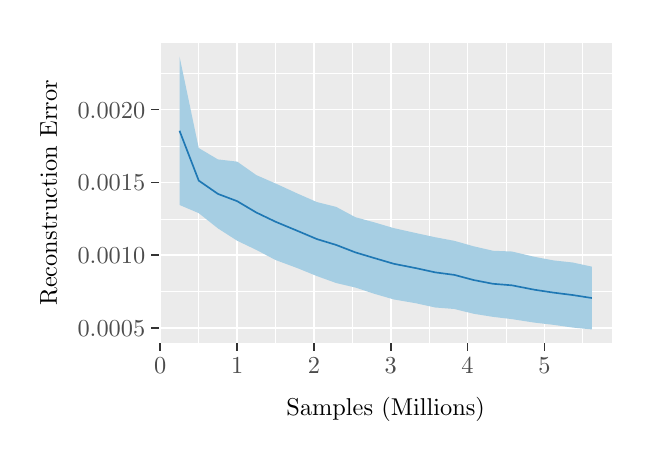
\begin{tikzpicture}[x=1pt,y=1pt]
\definecolor{fillColor}{RGB}{255,255,255}
\path[use as bounding box,fill=fillColor,fill opacity=0.00] (0,0) rectangle (216.81,144.54);
\begin{scope}
\path[clip] (  0.00,  0.00) rectangle (216.81,144.54);
\definecolor{drawColor}{RGB}{255,255,255}
\definecolor{fillColor}{RGB}{255,255,255}

\path[draw=drawColor,line width= 0.6pt,line join=round,line cap=round,fill=fillColor] (  0.00,  0.00) rectangle (216.81,144.54);
\end{scope}
\begin{scope}
\path[clip] ( 47.42, 30.57) rectangle (211.31,139.04);
\definecolor{fillColor}{gray}{0.92}

\path[fill=fillColor] ( 47.42, 30.57) rectangle (211.31,139.04);
\definecolor{drawColor}{RGB}{255,255,255}

\path[draw=drawColor,line width= 0.3pt,line join=round] ( 47.42, 49.12) --
	(211.31, 49.12);

\path[draw=drawColor,line width= 0.3pt,line join=round] ( 47.42, 75.43) --
	(211.31, 75.43);

\path[draw=drawColor,line width= 0.3pt,line join=round] ( 47.42,101.75) --
	(211.31,101.75);

\path[draw=drawColor,line width= 0.3pt,line join=round] ( 47.42,128.07) --
	(211.31,128.07);

\path[draw=drawColor,line width= 0.3pt,line join=round] ( 61.81, 30.57) --
	( 61.81,139.04);

\path[draw=drawColor,line width= 0.3pt,line join=round] ( 89.57, 30.57) --
	( 89.57,139.04);

\path[draw=drawColor,line width= 0.3pt,line join=round] (117.32, 30.57) --
	(117.32,139.04);

\path[draw=drawColor,line width= 0.3pt,line join=round] (145.08, 30.57) --
	(145.08,139.04);

\path[draw=drawColor,line width= 0.3pt,line join=round] (172.84, 30.57) --
	(172.84,139.04);

\path[draw=drawColor,line width= 0.3pt,line join=round] (200.60, 30.57) --
	(200.60,139.04);

\path[draw=drawColor,line width= 0.6pt,line join=round] ( 47.42, 35.96) --
	(211.31, 35.96);

\path[draw=drawColor,line width= 0.6pt,line join=round] ( 47.42, 62.28) --
	(211.31, 62.28);

\path[draw=drawColor,line width= 0.6pt,line join=round] ( 47.42, 88.59) --
	(211.31, 88.59);

\path[draw=drawColor,line width= 0.6pt,line join=round] ( 47.42,114.91) --
	(211.31,114.91);

\path[draw=drawColor,line width= 0.6pt,line join=round] ( 47.93, 30.57) --
	( 47.93,139.04);

\path[draw=drawColor,line width= 0.6pt,line join=round] ( 75.69, 30.57) --
	( 75.69,139.04);

\path[draw=drawColor,line width= 0.6pt,line join=round] (103.45, 30.57) --
	(103.45,139.04);

\path[draw=drawColor,line width= 0.6pt,line join=round] (131.20, 30.57) --
	(131.20,139.04);

\path[draw=drawColor,line width= 0.6pt,line join=round] (158.96, 30.57) --
	(158.96,139.04);

\path[draw=drawColor,line width= 0.6pt,line join=round] (186.72, 30.57) --
	(186.72,139.04);
\definecolor{fillColor}{RGB}{166,206,227}

\path[fill=fillColor] ( 54.87,134.11) --
	( 61.81,101.05) --
	( 68.75, 96.93) --
	( 75.69, 96.14) --
	( 82.63, 91.26) --
	( 89.57, 88.24) --
	( 97.60, 84.55) --
	(104.53, 81.51) --
	(111.47, 79.78) --
	(118.41, 76.05) --
	(125.35, 74.16) --
	(132.29, 72.10) --
	(140.32, 70.32) --
	(147.26, 68.81) --
	(154.20, 67.51) --
	(161.14, 65.54) --
	(168.08, 63.94) --
	(175.01, 63.65) --
	(183.04, 61.75) --
	(189.98, 60.44) --
	(196.92, 59.69) --
	(203.86, 58.19) --
	(203.86, 35.50) --
	(196.92, 36.18) --
	(189.98, 37.16) --
	(183.04, 37.97) --
	(175.01, 39.22) --
	(168.08, 40.05) --
	(161.14, 41.16) --
	(154.20, 42.88) --
	(147.26, 43.43) --
	(140.32, 44.95) --
	(132.29, 46.34) --
	(125.35, 48.35) --
	(118.41, 50.64) --
	(111.47, 52.27) --
	(104.53, 54.77) --
	( 97.60, 57.60) --
	( 89.57, 60.58) --
	( 82.63, 64.23) --
	( 75.69, 67.56) --
	( 68.75, 72.01) --
	( 61.81, 77.52) --
	( 54.87, 80.47) --
	cycle;
\definecolor{drawColor}{RGB}{31,120,180}

\path[draw=drawColor,line width= 0.6pt,line join=round] ( 54.87,107.29) --
	( 61.81, 89.28) --
	( 68.75, 84.47) --
	( 75.69, 81.85) --
	( 82.63, 77.74) --
	( 89.57, 74.41) --
	( 97.60, 71.07) --
	(104.53, 68.14) --
	(111.47, 66.03) --
	(118.41, 63.34) --
	(125.35, 61.26) --
	(132.29, 59.22) --
	(140.32, 57.64) --
	(147.26, 56.12) --
	(154.20, 55.20) --
	(161.14, 53.35) --
	(168.08, 52.00) --
	(175.01, 51.43) --
	(183.04, 49.86) --
	(189.98, 48.80) --
	(196.92, 47.93) --
	(203.86, 46.85);
\end{scope}
\begin{scope}
\path[clip] (  0.00,  0.00) rectangle (216.81,144.54);
\definecolor{drawColor}{gray}{0.30}

\node[text=drawColor,anchor=base east,inner sep=0pt, outer sep=0pt, scale=  0.88] at ( 42.47, 32.93) {0.0005};

\node[text=drawColor,anchor=base east,inner sep=0pt, outer sep=0pt, scale=  0.88] at ( 42.47, 59.24) {0.0010};

\node[text=drawColor,anchor=base east,inner sep=0pt, outer sep=0pt, scale=  0.88] at ( 42.47, 85.56) {0.0015};

\node[text=drawColor,anchor=base east,inner sep=0pt, outer sep=0pt, scale=  0.88] at ( 42.47,111.88) {0.0020};
\end{scope}
\begin{scope}
\path[clip] (  0.00,  0.00) rectangle (216.81,144.54);
\definecolor{drawColor}{gray}{0.20}

\path[draw=drawColor,line width= 0.6pt,line join=round] ( 44.67, 35.96) --
	( 47.42, 35.96);

\path[draw=drawColor,line width= 0.6pt,line join=round] ( 44.67, 62.28) --
	( 47.42, 62.28);

\path[draw=drawColor,line width= 0.6pt,line join=round] ( 44.67, 88.59) --
	( 47.42, 88.59);

\path[draw=drawColor,line width= 0.6pt,line join=round] ( 44.67,114.91) --
	( 47.42,114.91);
\end{scope}
\begin{scope}
\path[clip] (  0.00,  0.00) rectangle (216.81,144.54);
\definecolor{drawColor}{gray}{0.20}

\path[draw=drawColor,line width= 0.6pt,line join=round] ( 47.93, 27.82) --
	( 47.93, 30.57);

\path[draw=drawColor,line width= 0.6pt,line join=round] ( 75.69, 27.82) --
	( 75.69, 30.57);

\path[draw=drawColor,line width= 0.6pt,line join=round] (103.45, 27.82) --
	(103.45, 30.57);

\path[draw=drawColor,line width= 0.6pt,line join=round] (131.20, 27.82) --
	(131.20, 30.57);

\path[draw=drawColor,line width= 0.6pt,line join=round] (158.96, 27.82) --
	(158.96, 30.57);

\path[draw=drawColor,line width= 0.6pt,line join=round] (186.72, 27.82) --
	(186.72, 30.57);
\end{scope}
\begin{scope}
\path[clip] (  0.00,  0.00) rectangle (216.81,144.54);
\definecolor{drawColor}{gray}{0.30}

\node[text=drawColor,anchor=base,inner sep=0pt, outer sep=0pt, scale=  0.88] at ( 47.93, 19.56) {0};

\node[text=drawColor,anchor=base,inner sep=0pt, outer sep=0pt, scale=  0.88] at ( 75.69, 19.56) {1};

\node[text=drawColor,anchor=base,inner sep=0pt, outer sep=0pt, scale=  0.88] at (103.45, 19.56) {2};

\node[text=drawColor,anchor=base,inner sep=0pt, outer sep=0pt, scale=  0.88] at (131.20, 19.56) {3};

\node[text=drawColor,anchor=base,inner sep=0pt, outer sep=0pt, scale=  0.88] at (158.96, 19.56) {4};

\node[text=drawColor,anchor=base,inner sep=0pt, outer sep=0pt, scale=  0.88] at (186.72, 19.56) {5};
\end{scope}
\begin{scope}
\path[clip] (  0.00,  0.00) rectangle (216.81,144.54);
\definecolor{drawColor}{RGB}{0,0,0}

\node[text=drawColor,anchor=base,inner sep=0pt, outer sep=0pt, scale=  0.88] at (129.37,  4.25) {Samples (Millions)};
\end{scope}
\begin{scope}
\path[clip] (  0.00,  0.00) rectangle (216.81,144.54);
\definecolor{drawColor}{RGB}{0,0,0}

\node[text=drawColor,rotate= 90.00,anchor=base,inner sep=0pt, outer sep=0pt, scale=  0.88] at ( 10.59, 84.81) {Reconstruction Error};
\end{scope}
\end{tikzpicture}
